\chapter{Ergebnisse} % (fold)
\label{sec:ergebnisse}
Im Nachfolgenden werden die Ergebnisse der Latenztests der oben eingeführten APIs dargestellt.

\noindent
Wie in Abbildung 7.1 zusehen ist, hat die PostgreSQL REST-API eine höhere Latenzzeit als die GraphQL PostgeSQL. Dies deutet darauf hin, dass die GraphQL API bei der Abfrage eines spezifischen Personenobjekts, anhand der Personen-ID in kombination mit einer relationalen Datenbank effizientere Abfragen und eine bessere Performance bei der Verarbeitung bietet. Ähnliches zeigt sich bei einer Neo4j Datenbank. Auch hier hat die Neo4j GraphQL API niedrigere Latenzzeiten als die REST-API. Allerdings sind die Latenzen bei Neo4j minimal höher als bei dem realtionalen Pendant. Das deutet darauf hin, dass Postgres bei dieser Anfrage eine performantere Verarbeitung von Abfragen ermöglicht. Zusammenfassend kann man für diese Anfrage sagen, dass GraphQL sowohl in kombination mit einer relationalen, als auch einer Graphdatenbank eine niedrigere Latenz aufweist. Zudem ist Postgres bei dieser Anfrage insgesamt ein wenig performanter als neo4j.
\newline
In Abbildung 7.2 sind die Latenzen für die komplexere Anfrge, die alle Personenobjekte aus der Datenbank zurückliefert dargestellt. Bei den APIs die mit Postgres implementiert sind ist eine deutlich niedrigere Latenz zu sehen, als bei den mit neo4j implementierten. GraphQL hat hierbei sowohl bei der relationalen Datenbank als auch bei der Graphdatenbank im Median eine niedrigere Latenz. REST ist somit in beiden Fällen die unperformantere API.
\newline
Wenn nun die Anfragekomplexität steigt, wodurch sich die Abhängigkeit zwischen den Objekten in der Datenbank erhöht, ist deutlich zu sehen, dass die Streuung bei der Postgres REST-API höher ist als bei allen anderen APIs (vgl Abb.7.3). Zudem ist diese API diejenige mit der höchsten Latenz. Allerdings liegt die Neo4j REST-API im Median über den Postgres REST-API. Beide GraphQL APIs weißen erneut eine deutlich niedrigere Latenz auf.
\newline
Bei der Speicherung in eine Datenbank ist ein deutlich anderes Bild zu sehen. Wie in Abbildung 7.4 zusehen, ist hierbei die Postgres REST-API diejenige mit der geringsten LAtenz. Dicht gefolgt von der Postgres GraphQL API. Eine deutlich höhere Latenz ist bei den neo4j APIs zu erkennen. Hierbei ist allerdings die GraphQL API die performantere.




\begin{figure}[htbp]
 \centering
	\begin{tikzpicture}
	    \begin{axis}[
	        boxplot/draw direction=y, 
	        xlabel={API}, 
	        ylabel={ms}, 
	        xtick={1,2,3,4}, 
	        xticklabels={Post Rest, Post Graph, Neo4 Rest, Neo4 Graph}, 
	        ymin=50, ymax=65,
	       ytick distance=1,
                  width=15cm,
	       height= 18cm
	    ]
	       \addplot+[
	            boxplot prepared={
	                median=52,
	                upper quartile=55,
	                lower quartile=52, 
	                upper whisker=59,
	                lower whisker=51
	            },
	            draw=black
	        ] coordinates {};
	        \addplot+[
	            boxplot prepared={
	                median=53,
	                upper quartile=53,
	                lower quartile=53, 
	                upper whisker=54,
	                lower whisker=52
	            },
	            draw=black
	        ] coordinates {};
	         \addplot+[
	            boxplot prepared={
	                median=52,
	                upper quartile=58,
	                lower quartile=52, 
	                upper whisker=63,
	                lower whisker=51
	            },
	            draw=black
	        ] coordinates {};
	       \addplot+[
	            boxplot prepared={
	                median=52,
	                upper quartile=53,
	                lower quartile=52, 
	                upper whisker=54,
	                lower whisker=51
	            },
	            draw=black
	        ] coordinates {};
	    \end{axis}
	\end{tikzpicture}
\caption{HEAD /api/resource}
\end{figure}




\begin{figure}
\centering
\begin{tikzpicture}[scale=1.9]
\begin{axis}[
    axis lines = middle,
    xlabel = {x},
    ylabel = {y},
    zlabel = {z},
    xmode = log,
    width=10cm,
    height=10cm,
    grid = major,
    enlarge x limits = true,
    view={0}{0},
    ymin=0, ymax=3,  
]
% Linie und Punkte für die ersten Punkte (rot)
\addplot3+[
    only marks, 
    mark=*,
    red,
    mark options={fill=red} % Innere des Punktes rot färben
] coordinates {
    (1, 0, 111)
    (100, 0, 121)
    (1000, 0, 135)
    (10000, 0, 272)
    (100000, 0, 426.5)
};
\addplot3[
    red, % Linie durch die Punkte
    mark=none % keine Markierungen an der Linie
] coordinates {
    (1, 0, 111)
    (100, 0, 121)
    (1000, 0, 135)
    (10000, 0, 272)
    (100000, 0, 426.5)
};
% Linie und Punkte für die zweiten Punkte (blau)
\addplot3+[
    only marks, 
    mark=square*,
    blue,
    mark options={fill=blue} % Innere des Punktes blau färben
] coordinates {
    (1, 1, 111)
    (100, 1, 122)
    (1000, 1, 134)
    (10000, 1, 271.5)
    (100000, 1, 468)
};
\addplot3[
    blue, % Linie durch die Punkte
    mark=none % keine Markierungen an der Linie
] coordinates {
    (1, 1, 111)
    (100, 1, 122)
    (1000, 1, 134)
    (10000, 1, 271.5)
    (100000, 1, 468)
};
% Linie und Punkte für die vierten Punkte (orange)
\addplot3+[
    only marks, 
    mark=diamond*,
    orange,
    mark options={fill=orange} % Innere des Punktes orange färben
] coordinates {
    (1, 3, 111)
    (100, 3, 119.5)
    (1000, 3, 146)
    (10000, 3, 267)
    (100000, 3, 492.5)
};
\addplot3[
    orange, % Linie durch die Punkte
    mark=none % keine Markierungen an der Linie
] coordinates {
    (1, 3, 111)
    (100, 3, 119.5)
    (1000, 3, 146)
    (10000, 3, 267)
    (100000, 3, 492.5)
};
\end{axis}
\end{tikzpicture}
\caption{PostREST parametriesierte Abfragen}
\end{figure}

\begin{figure}
\centering
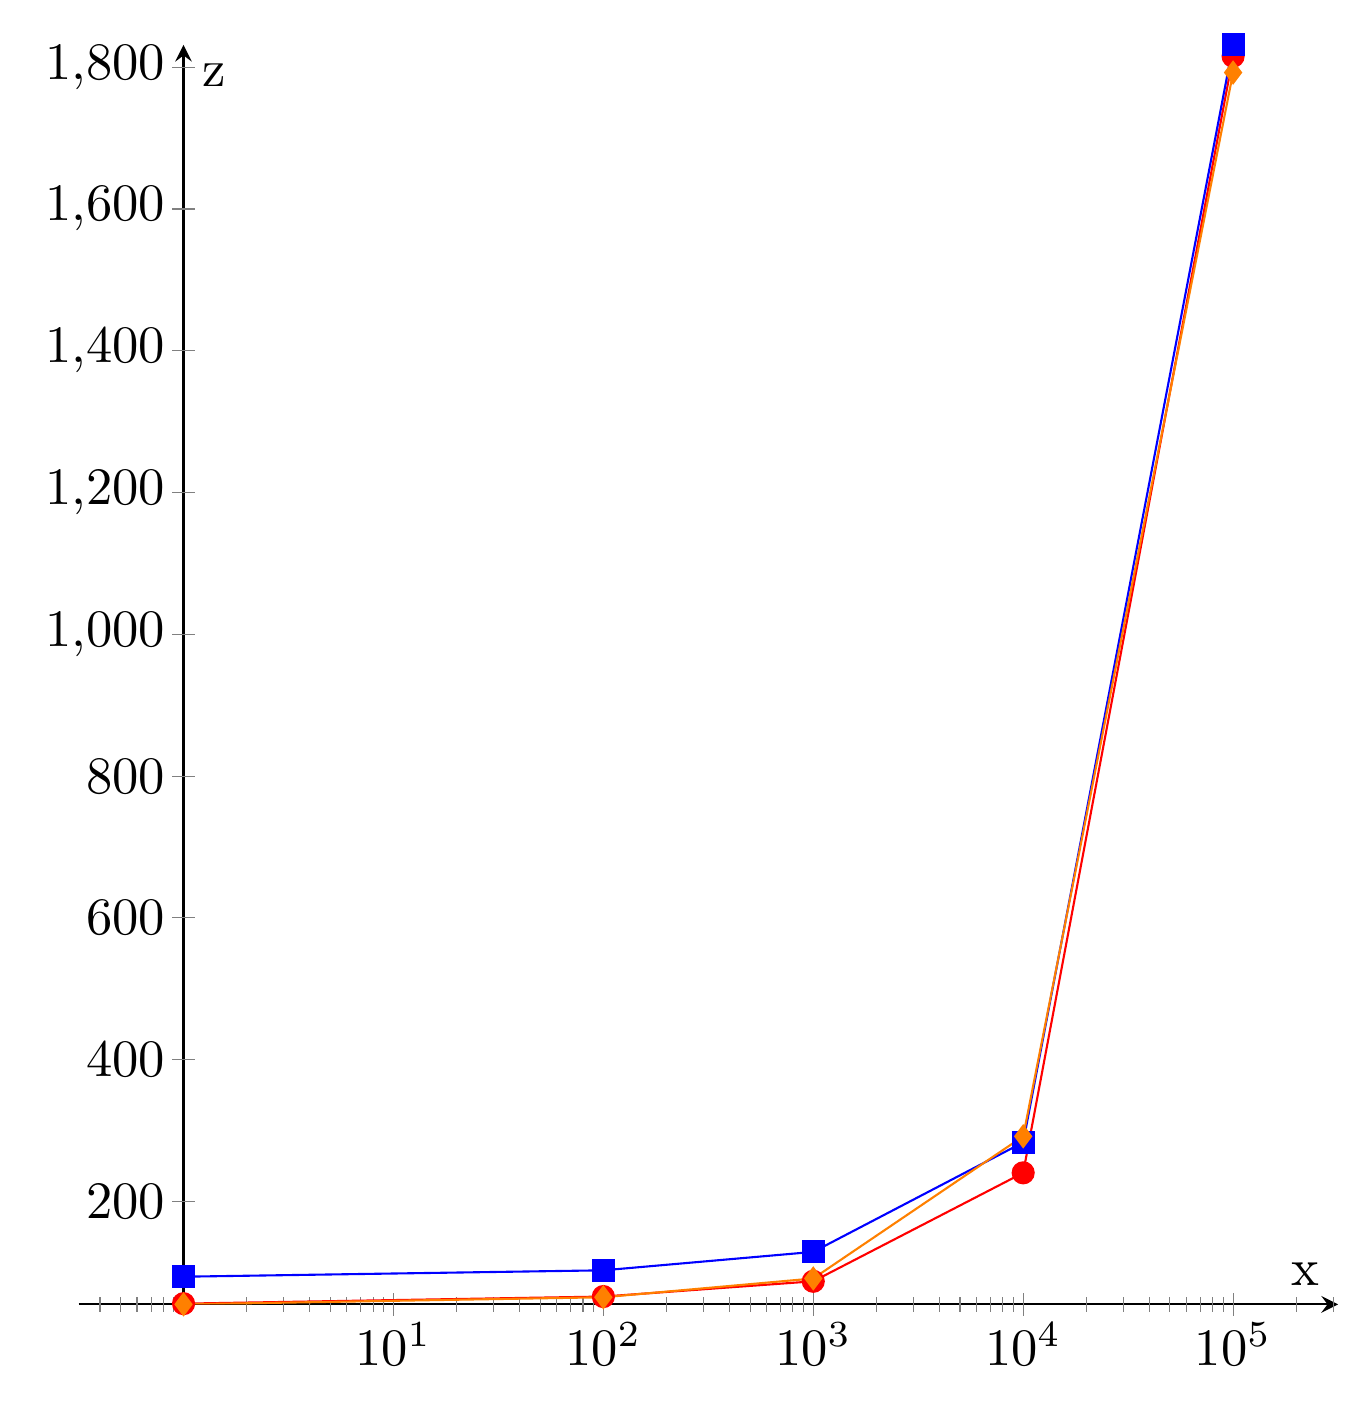
\begin{tikzpicture}[scale=1.9]
\begin{axis}[
    axis lines = middle,
    xlabel = {x},
    ylabel = {y},
    zlabel = {z},
    xmode = log,
    width=10cm,
    height=10cm,
    grid = major,
    enlarge x limits = true,
    view={0}{0},
    ymin=0, ymax=3,  
]
% Linie und Punkte für die ersten Punkte (rot)
\addplot3+[
    only marks, 
    mark=*,
    red,
    mark options={fill=red} % Innere des Punktes rot färben
] coordinates {
    (1, 0, 56)
    (100, 0, 66)
    (1000, 0, 87.5)
    (10000, 0, 240.5)
    (100000, 0, 1815.5)
};
\addplot3[
    red, % Linie durch die Punkte
    mark=none % keine Markierungen an der Linie
] coordinates {
    (1, 0, 56)
    (100, 0, 66)
    (1000, 0, 87.5)
    (10000, 0, 240.5)
    (100000, 0, 1815.5)
};
% Linie und Punkte für die zweiten Punkte (blau)
\addplot3+[
    only marks, 
    mark=square*,
    blue,
    mark options={fill=blue} % Innere des Punktes blau färben
] coordinates {
    (1, 1, 94)
    (100, 1, 103)
    (1000, 1, 129)
    (10000, 1, 283.5)
    (100000, 1, 1831.5)
};
\addplot3[
    blue, % Linie durch die Punkte
    mark=none % keine Markierungen an der Linie
] coordinates {
    (1, 1, 94)
    (100, 1, 103)
    (1000, 1, 129)
    (10000, 1, 283.5)
    (100000, 1, 1831.5)
};
% Linie und Punkte für die vierten Punkte (orange)
\addplot3+[
    only marks, 
    mark=diamond*,
    orange,
    mark options={fill=orange} % Innere des Punktes orange färben
] coordinates {
    (1, 3, 55)
    (100, 3, 65)
    (1000, 3, 91.5)
    (10000, 3, 292)
    (100000, 3, 1792.5)
};
\addplot3[
    orange, % Linie durch die Punkte
    mark=none % keine Markierungen an der Linie
] coordinates {
    (1, 3, 55)
    (100, 3, 65)
    (1000, 3, 91.5)
    (10000, 3, 292)
    (100000, 3, 1792.5)
};
\end{axis}
\end{tikzpicture}
\caption{PostGraph parametriesierte Abfragen}
\end{figure}



\begin{figure}
\centering
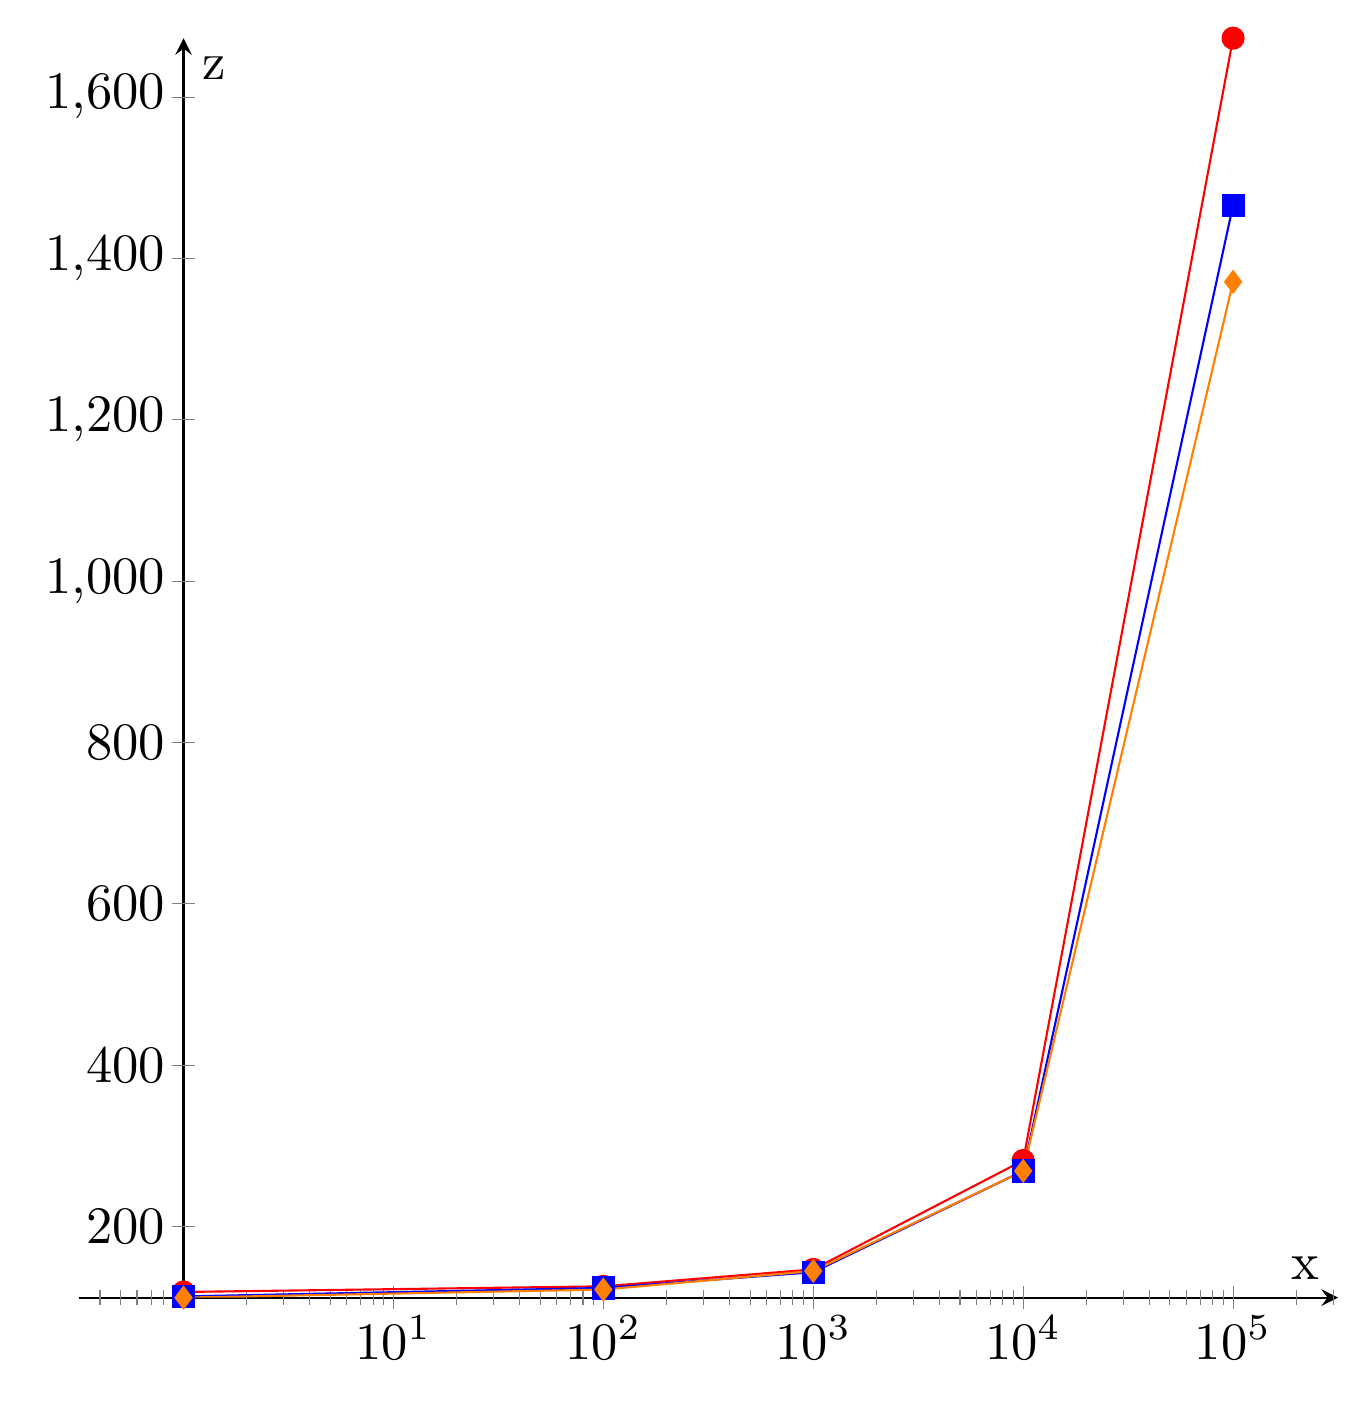
\begin{tikzpicture}[scale=1.9]
\begin{axis}[
    axis lines = middle,
    xlabel = {x},
    ylabel = {y},
    zlabel = {z},
    xmode = log,
    width=10cm,
    height=10cm,
    grid = major,
    enlarge x limits = true,
    view={0}{0},
    ymin=0, ymax=3,  
]
% Linie und Punkte für die ersten Punkte (rot)
\addplot3+[
    only marks, 
    mark=*,
    red,
    mark options={fill=red} % Innere des Punktes rot färben
] coordinates {
    (1, 0, 119)
    (100, 0, 126)
    (1000, 0, 147)
    (10000, 0, 282)
    (100000, 0, 1673)
};
\addplot3[
    red, % Linie durch die Punkte
    mark=none % keine Markierungen an der Linie
] coordinates {
    (1, 0, 119)
    (100, 0, 126)
    (1000, 0, 147)
    (10000, 0, 282)
    (100000, 0,1673)
};
% Linie und Punkte für die zweiten Punkte (blau)
\addplot3+[
    only marks, 
    mark=square*,
    blue,
    mark options={fill=blue} % Innere des Punktes blau färben
] coordinates {
    (1, 1, 113.5)
    (100, 1, 124)
    (1000, 1, 143.5)
    (10000, 1, 269)
    (100000, 1, 1466)
};
\addplot3[
    blue, % Linie durch die Punkte
    mark=none % keine Markierungen an der Linie
] coordinates {
    (1, 1, 113.5)
    (100, 1, 124)
    (1000, 1, 143.5)
    (10000, 1, 269)
    (100000, 1, 1466)
};
% Linie und Punkte für die vierten Punkte (orange)
\addplot3+[
    only marks, 
    mark=diamond*,
    orange,
    mark options={fill=orange} % Innere des Punktes orange färben
] coordinates {
    (1, 3, 112)
    (100, 3, 122)
    (1000, 3, 145)
    (10000, 3, 269)
    (100000, 3, 1371)
};
\addplot3[
    orange, % Linie durch die Punkte
    mark=none % keine Markierungen an der Linie
] coordinates {
    (1, 3, 112)
    (100, 3, 122)
    (1000, 3, 145)
    (10000, 3, 269)
    (100000, 3, 1371)
};
\end{axis}
\end{tikzpicture}
\caption{Neo4REST parametriesierte Abfragen}
\end{figure}


\begin{figure}
\centering
\begin{tikzpicture}[scale=1.9]
\begin{axis}[
    axis lines = middle,
    xlabel = {x},
    ylabel = {y},
    zlabel = {z},
    xmode = log,
    width=10cm,
    height=10cm,
    grid = major,
    enlarge x limits = true,
    view={0}{0},
    ymin=0, ymax=3,  
]
% Linie und Punkte für die ersten Punkte (rot)
\addplot3+[
    only marks, 
    mark=*,
    red,
    mark options={fill=red} % Innere des Punktes rot färben
] coordinates {
    (1, 0, 58)
    (100, 0, 70)
    (1000, 0, 105.5)
    (10000, 0, 391)
    (100000, 0, 2726.5)
};
\addplot3[
    red, % Linie durch die Punkte
    mark=none % keine Markierungen an der Linie
] coordinates {
    (1, 0, 58)
    (100, 0, 70)
    (1000, 0, 105.5)
    (10000, 0, 391)
    (100000, 0,2726.5)
};
% Linie und Punkte für die zweiten Punkte (blau)
\addplot3+[
    only marks, 
    mark=square*,
    blue,
    mark options={fill=blue} % Innere des Punktes blau färben
] coordinates {
    (1, 1, 59)
    (100, 1, 70)
    (1000, 1, 102.5)
    (10000, 1, 330)
    (100000, 1, 2484.5)
};
\addplot3[
    blue, % Linie durch die Punkte
    mark=none % keine Markierungen an der Linie
] coordinates {
    (1, 1, 59)
    (100, 1, 70)
    (1000, 1, 102.5)
    (10000, 1, 330)
    (100000, 1, 2484.5)
};
% Linie und Punkte für die vierten Punkte (orange)
\addplot3+[
    only marks, 
    mark=diamond*,
    orange,
    mark options={fill=orange} % Innere des Punktes orange färben
] coordinates {
    (1, 3, 57)
    (100, 3, 69)
    (1000, 3, 96)
    (10000, 3, 317)
    (100000, 3, 2396.5)
};
\addplot3[
    orange, % Linie durch die Punkte
    mark=none % keine Markierungen an der Linie
] coordinates {
    (1, 3, 57)
    (100, 3, 69)
    (1000, 3, 96)
    (10000, 3, 317)
    (100000, 3, 2396.5)
};
\end{axis}
\end{tikzpicture}
\caption{Neo4Graph parametriesierte Abfragen}
\end{figure}















\begin{figure}[htbp]
 \centering
	\begin{tikzpicture}
	    \begin{axis}[
	        boxplot/draw direction=y, 
	        xlabel={API}, 
	        ylabel={ms}, 
	        ytick distance=5,
	        xtick={1,2,3,4}, 
	        xticklabels={Post Rest, Post Graph, Neo4 Rest, Neo4 Graph}, 
	        ymin=50, ymax=150,
		width=15cm,
		height= 18cm
	    ]
	        \addplot+[
	            boxplot prepared={
	                median=109,
	                upper quartile=110,
	                lower quartile=108, 
	                upper whisker=113,
	                lower whisker=107
	            },
	            draw=black
	        ] coordinates {};
	        \addplot+[
	            boxplot prepared={
	                median=56,
	                upper quartile=58,
	                lower quartile=56, 
	                upper whisker=60,
	                lower whisker=54
	            },
	            draw=black
	        ] coordinates {};
	        \addplot+[
	            boxplot prepared={
	                median=113,
	                upper quartile=115,
	                lower quartile=111, 
	                upper whisker=119,
	                lower whisker=110
	            },
	            draw=black
	        ] coordinates {};
	       \addplot+[
	            boxplot prepared={
	                median=58,
	                upper quartile=59,
	                lower quartile=57, 
	                upper whisker=62,
	                lower whisker=56
	            },
	            draw=black
	        ] coordinates {};
	    \end{axis}
	\end{tikzpicture}
\caption{GET /api/persons/:pid}
\end{figure}

\begin{figure}[htbp]
 \centering
	\begin{tikzpicture}
	    \begin{axis}[
	        boxplot/draw direction=y, 
	        xlabel={API}, 
	        ylabel={ms}, 
	        xtick={1,2,3,4}, 
	        xticklabels={Post Rest, Post Graph, Neo4 Rest, Neo4 Graph}, 
	        ymin=50, ymax=590,
                  ytick distance=20,
                  width=15cm,
	       height= 18cm
	    ]
	        \addplot+[
	            boxplot prepared={
	                median=264,
	                upper quartile=274,
	                lower quartile=259, 
	                upper whisker=293,
	                lower whisker=237
	            },
	            draw=black
	        ] coordinates {};
	        \addplot+[
	            boxplot prepared={
	                median=206,
	                upper quartile=214,
	                lower quartile=198, 
	                upper whisker=233,
	                lower whisker=178
	            },
	            draw=black
	        ] coordinates {};
	         \addplot+[
	            boxplot prepared={
	                median=539,
	                upper quartile=551,
	                lower quartile=529, 
	                upper whisker=579,
	                lower whisker=499
	            },
	            draw=black
	        ] coordinates {};
	       \addplot+[
	            boxplot prepared={
	                median=499,
	                upper quartile=509,
	                lower quartile=494, 
	                upper whisker=531,
	                lower whisker=482
	            },
	            draw=black
	        ] coordinates {};
	    \end{axis}
	\end{tikzpicture}
\caption{GET /api/persons}
\end{figure}

\begin{figure}[htbp]
 \centering
	\begin{tikzpicture}
	    \begin{axis}[
	        boxplot/draw direction=y, 
	        xlabel={API}, 
	        ylabel={ms}, 
	        xtick={1,2,3,4}, 
	        xticklabels={Post Rest, Post Graph, Neo4 Rest, Neo4 Graph}, 
	        ymin=50, ymax=140,
	        ytick distance=5,
                  width=15cm,
	       height= 18cm
	    ]
	        \addplot+[
	            boxplot prepared={
	                median=111,
	                upper quartile=119,
	                lower quartile=109, 
	                upper whisker=134,
	                lower whisker=107
	            },
	            draw=black
	        ] coordinates {};
	        \addplot+[
	            boxplot prepared={
	                median=56,
	                upper quartile=57,
	                lower quartile=56, 
	                upper whisker=58,
	                lower whisker=55
	            },
	            draw=black
	        ] coordinates {};
	         \addplot+[
	            boxplot prepared={
	                median=115,
	                upper quartile=117,
	                lower quartile=113, 
	                upper whisker=123,
	                lower whisker=111
	            },
	            draw=black
	        ] coordinates {};
	       \addplot+[
	            boxplot prepared={
	                median=57,
	                upper quartile=58,
	                lower quartile=56, 
	                upper whisker=59,
	                lower whisker=55
	            },
	            draw=black
	        ] coordinates {};
	    \end{axis}
	\end{tikzpicture}
\caption{GET /api/persons/:pid/projects/issues}
\end{figure}

\begin{figure}[htbp]
 \centering
	\begin{tikzpicture}
	    \begin{axis}[
	        boxplot/draw direction=y, 
	        xlabel={API}, 
	        ylabel={ms}, 
	        xtick={1,2,3,4}, 
	        xticklabels={Post Rest, Post Graph, Neo4 Rest, Neo4 Graph}, 
	        ymin=50, ymax=130,
	       ytick distance=5,
                  width=15cm,
	       height= 18cm
	    ]
	       \addplot+[
	            boxplot prepared={
	                median=56,
	                upper quartile=57,
	                lower quartile=55, 
	                upper whisker=60,
	                lower whisker=54
	            },
	            draw=black
	        ] coordinates {};
	        \addplot+[
	            boxplot prepared={
	                median=58,
	                upper quartile=60,
	                lower quartile=57, 
	                upper whisker=62,
	                lower whisker=55
	            },
	            draw=black
	        ] coordinates {};
	         \addplot+[
	            boxplot prepared={
	                median=89,
	                upper quartile=97,
	                lower quartile=83, 
	                upper whisker=118,
	                lower whisker=77
	            },
	            draw=black
	        ] coordinates {};
	       \addplot+[
	            boxplot prepared={
	                median=82,
	                upper quartile=87,
	                lower quartile=78, 
	                upper whisker=99,
	                lower whisker=73
	            },
	            draw=black
	        ] coordinates {};
	    \end{axis}
	\end{tikzpicture}
\caption{POST /api/persons/:pid/projects/:prid/issues}
\end{figure}

% chapter ergebnisse (end)